
CMake的构建过程分为两步,如下图所示。首先,若使用时没有特殊标志,CMake会在配置过程中扫描系统中可用的工具链,再决定输出。第二步是调用\texttt{cmake -{}-build}时的实际编译和构建:

\begin{center}
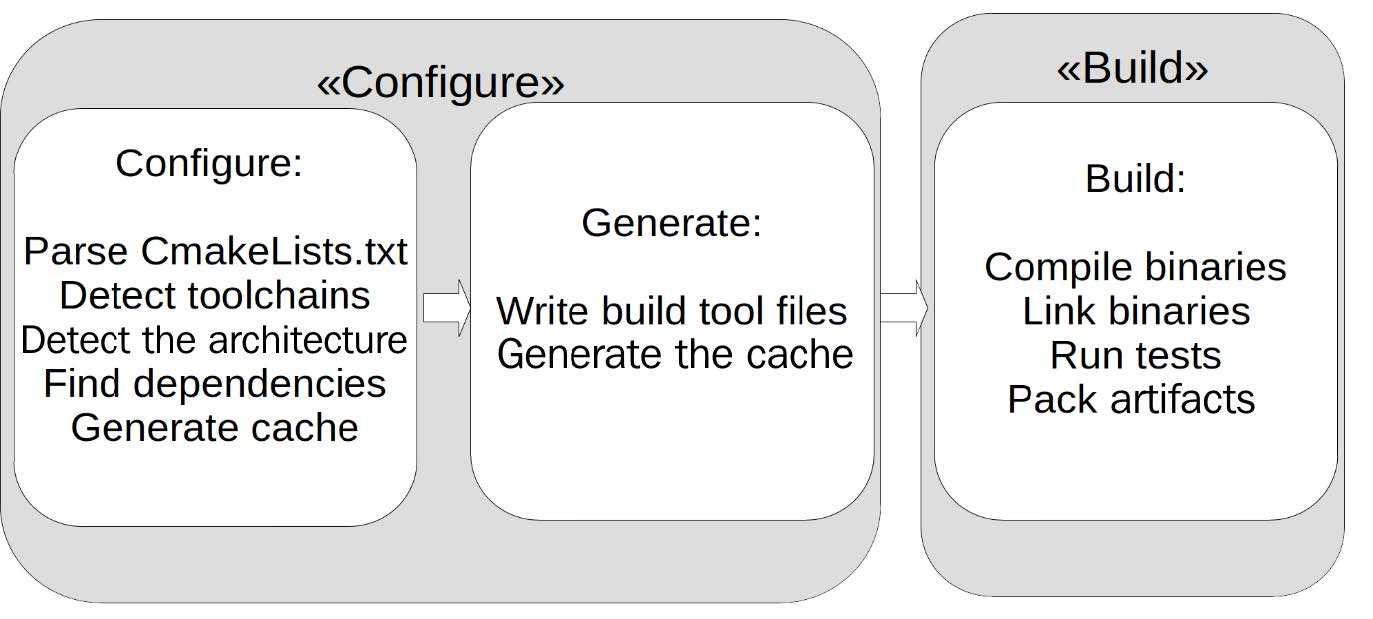
\includegraphics[width=0.6\textwidth]{content/1/chapter1/images/3.jpg}\\
图1.3  CMake的两阶段构建过程
\end{center}

标准输出是Unix Makefiles,除非检测到唯一的编译器是Microsoft Visual Studio,这种情况下将创建Visual Studio解决方案(.sln)。

修改生成器,可以使用\texttt{-G}选项:

\begin{tcblisting}{commandshell={}}
cmake .. -G Ninja
\end{tcblisting}

这将生成Ninja(\url{https://ninja-build.org/})的构建文件。CMake支持很多生成器,Ninja是其中之一。在CMake网站上可以找到一个生成器支持列表:\url{https://cmake.org/cmake/help/latest/manual/cmake-generators.7.html}.

生成器主要有两种类型——一种是Makefile风格的生成器和Ninja生成器,多以命令行方式使用,另一种是为IDE(如Visual Studio或Xcode)创建构建工程文件。

这里,CMake会区分单配置生成器和多配置生成器。对于单配置生成器,必须在每次更改配置时重写构建文件;多配置构建系统可以自行管理不同的配置,不需要重新生成。尽管本书中的示例使用的是单配置生成器,但它们也适用于多配置生成器。对于大多数示例,所选生成器是无关紧要的(否则,就会特别说明):

\begin{table}[H]
	\centering
	\begin{tabular}{|l|l|}
		\hline
		\textbf{生成器}                                                                                                                  &  \textbf{多配置}                                                            \\ \hline
		Makefile(所有版本)                                                                                                                                  &                                                                           No       \\  \hline
		Ninja              &                                                                                  No\\  \hline
		Ninja Multi-Config  &  Yes                                                                                \\ \hline
    Xcode              &                                                                                  Yes\\  \hline
    Visual Studio              &                                                                                  Yes\\  \hline
	\end{tabular}
\end{table}

此外,还有一些生成器,可以为编辑器或IDE生成项目信息,如Sublime Text 2、Kate editor、Code::Blocks和Eclipse。对于每个应用,可以选择编辑器或IDE使用Make,还是Ninja进行内部构建。

构建完成后,CMake将在构建文件夹中多了许多文件,其中最重要的就是CMakeCache.txt,其存储了所有检测到的配置。注意,当使用\texttt{cmake-gui}时,第一步会分为配置项目和生成构建文件。但当以命令行运行时,这些步骤合并为一个。配置完成后,将在构建文件夹执行构建。

\subsubsubsection{1.5.1\hspace{0.2cm}源文件夹和构建文件夹}

CMake中存在两个逻辑文件夹。一个是源文件夹,包含项目的层次结构集;另一个是构建文件夹,包含构建指令、缓存,以及所有生成的二进制文件和工件。

源文件夹是CMakeLists.txt文件所在的位置。构建文件夹可以放在源文件夹中,也可以将其放在另一个位置。两种方式都可以;注意,对于本书中的示例,我们决定将构建文件夹放在源文件夹中。构建文件夹通命名为\texttt{build},但也可以使用其他名称,包括不同平台的前缀和后缀。当在源代码树中使用构建文件夹时,最好将其添加到.gitignore中。

当配置CMake项目时,将在构建文件夹中重新创建源文件夹的项目和文件夹结构,以便所有构建工件都位于相同的位置。每个文件夹中,都有一个名为CMakeFiles的子文件夹,其中包含CMake配置步骤生成的信息。

下面显示了一个CMake项目的目录结构:

\begin{tcblisting}{commandshell={}}
.
├── simple_executable
│      ├── CMakeLists.txt
│      └── src
│            └── main.cpp
├── CMakeLists.txt
\end{tcblisting}

当执行CMake配置时,CMake项目的文件结构会映射到build文件夹中。每个包含CMakeLists.txt文件的文件夹将进行映射,将创建一个名为CMakeFiles的子文件夹,其中包含用于构建的信息:

\begin{tcblisting}{commandshell={}}
├── build
│     ├── simple_executable
│     │      └── CMakeFiles
│     └── CMakeFiles
\end{tcblisting}

我们已经使用已有项目来学习了CMake构建过程。了解了配置和构建步骤以及生成器,我们需要CMakeLists.txt文件来传递必要的信息给CMake。接下来,了解一下CMakeLists.txt文件怎么写,以及CMake语言如何工作。























